\documentclass{standalone}
\usepackage{tikz}

\begin{document}
	\tikzset{
	font=\footnotesize,
	minimum width=20
		}
	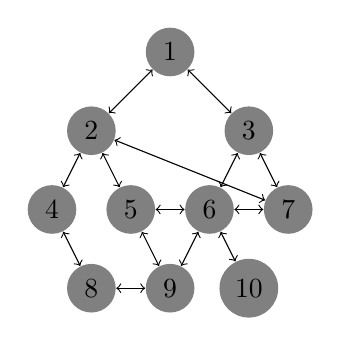
\begin{tikzpicture}
		\node[shape=circle,fill=gray] (a) at (10,0) {1};
	%	\node[shape=circle,fill=gray] (h) at (10.75,0) {2};
		\node[shape=circle,fill=gray] (b) at (9,-1) {2};
		\node[shape=circle,fill=gray] (c) at (11,-1) {3};
		\node[shape=circle,fill=gray] (d) at (8.5,-2) {4};
		\node[shape=circle,fill=gray] (e) at (9.5,-2) {5};
		\node[shape=circle,fill=gray] (f) at (10.5,-2) {6};
		\node[shape=circle,fill=gray] (g) at (11.5,-2) {7};
		\node[shape=circle,fill=gray] (x) at (9,-3) {8};
		\node[shape=circle,fill=gray] (y) at (10,-3) {9};
		\node[shape=circle,fill=gray] (z) at (11,-3) {10};
		\draw (a) edge[<->] (b) (a) edge[<->] (c) 	
	%	(h) edge[<->] (c)
		(b) edge[<->] (d)  (b) edge[<->] (g)
		(c) edge[<->] (f) (c) edge[<->] (g)
		(b) edge[<->] (e) (e) edge[<->] (f) (f) edge[<->] (g)
		(d) edge[<->] (x) (e) edge[<->] (y) (f) edge[<->] (z) (f) edge[<->] (y)
		(x) edge[<->] (y); 
	\end{tikzpicture}
\end{document}  